
\subsection{One-dimensional uniform dataset}

% We train a two-dimensional map over $25000$ samples drawn from a uniform distribution ($\mathcal{U}(0, 1)$). The map consists of $1024$ units (neurons) and it is being trained for $25000$ epochs (all the parameters can be found in Table~\ref{table:parameters}). Figure~\ref{fig:one-dim}{\bfseries \sffamily A} shows the neural space topology of the two-dimensional map after sampling a blue noise distribution and placing the neurons on the corresponding nodes. Figure~\ref{fig:one-dim}{\bfseries \sffamily B} indicates the learned representations after training. In this case the mapping of real numbers within the interval $[0, 1]$ is illustrated in color-code with blue color representing number zero and yellow representing one. It is clear that the map has organize the representations in a descending order starting from the upper left corner (one) of the map to the lower right corner (zero).

% Neurons of both the Kohonen and VSOM maps develop receptive filters during training. Each of these receptive fields usually captures a portion of the input space and learns the reciprocal representations. Therefore, we examine the receptive fields of neurons by evaluating their response to a stimulus. To this end, we feed the map with $6$ input samples after discretizing the interval $[0, 1]$. The activity of each neuron is  computed as the Euclidean distance between the input sample and the neuron's code word. Figures~\ref{fig:one-dim} {\sffamily \bfseries C}-{\sffamily \bfseries H}  show the neural activity on the map for $6$ input samples. It is apparent that different regions of the map respond to different stimuli, implying that the topographic organization has been successfully accomplished. 


\begin{figure}
  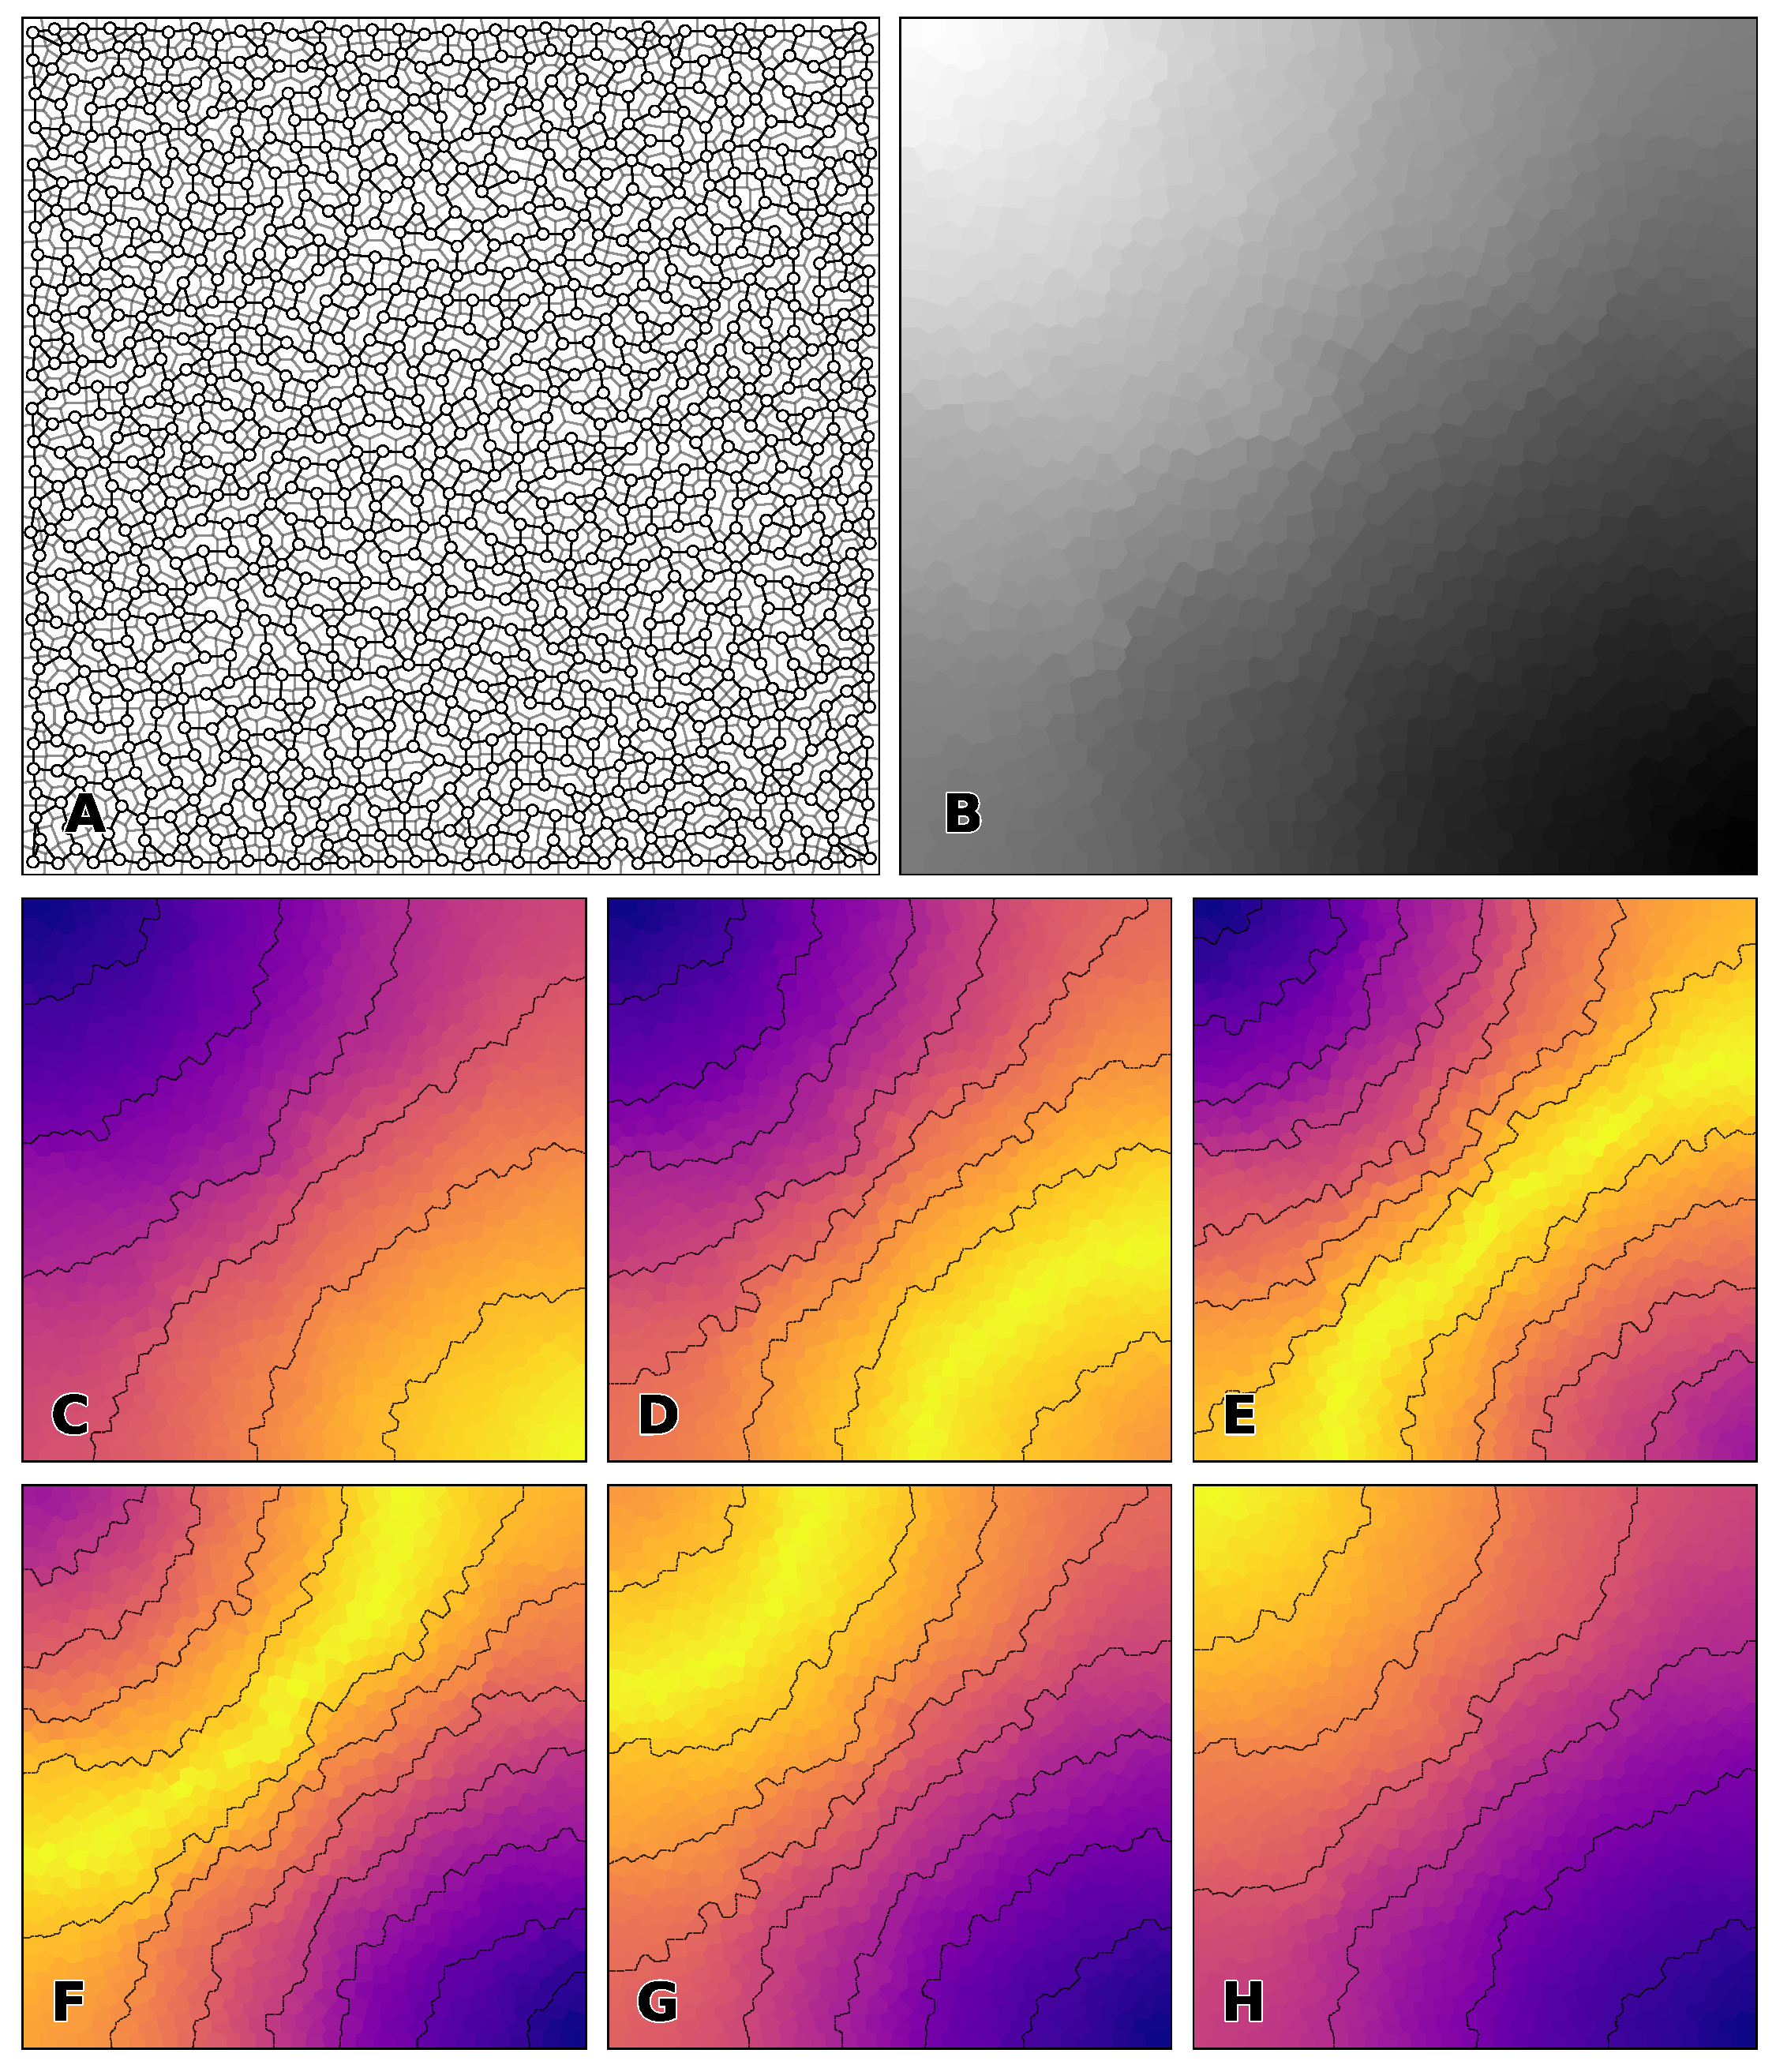
\includegraphics[width=\columnwidth]{experiment-1D-uniform.pdf}
  \vspace{2mm}
  \centering
  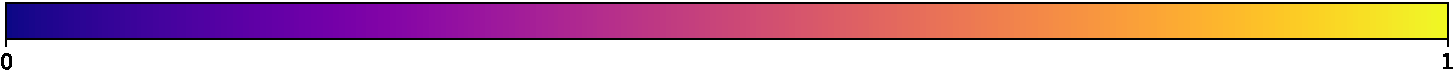
\includegraphics[width=.975\columnwidth]{figures/colormap.pdf}
  %
  \caption{%
  %
  {\bfseries \sffamily One dimensional uniform dataset with holes (results)}
  %
  Randomized SOM made of $1024$ neurons with a $3$-nearest neighbors induced topology. Model has been trained for $25,000$ epochs on one-dimensional points drawn from a uniform distribution on the unit segment. \textbf{A} Map topology in neural space. \textbf{B} Map topology in data space. \textbf{C to H} Receptive field of the map for six samples.
  %
  }
  \label{fig:1D-uniform:results}
\end{figure}
